\section{Detection sensitivity with Advanced gravitational wave detectors}
\label{sec:results}

To estimate how accurately we can infer the time evolution of $r=M_{\rm PNS}/R_{\rm PNS}^2$ in the
gravitational wave detector data, we have added {\tt s20-gw-10kpc} GW signal to 
Gaussian noise realisations whose power spectral density follows advanced LIGO
spectrum~\cite{aLIGOsens:2018} shown on Figure~\ref{fig:spectrum}. 
We have varied the distance to the source, covering a large
range of distances for which a detection in second generation of gravitational wave detectors
is feasible. The source is optimally oriented with
respect to the gravitational wave detector. We are assuming a GW signal from a core collapse
phenomena has been identified in the data and that the beginning of the GW signal is known within $O(10~ms)$.
The data (signal embedded in noise) are whitened using the function {\it prewhiten} of the R-package TSA.
An auto-regressive model with maximal \textcolor{red}{100} coefficients has been used.    

For each of the noise realisations, we reconstruct the ratio time series {$r_i$}
of length $N$ and compute two quantities that compare {$r_i$} to ratio {$r_i^0$} derived from
the PNS mass and radius generated by the simulation code that produces {\tt s20-gw-10kpc}.

The first quantity, $coverage$, is the fraction of the
ratio {$r_i^0$} values that fall within the 95\% confidence interval of {$r_i$}.
We also compute the $precision$ value given by
\begin{equation}
precision=\sum_1^N\frac{|r_i-r_i^0|}{r_i^0}
\end{equation}

Figure \ref{fig:s20results} is showing the median of $coverage$ and $precision$ as
function of the distance of the source as well as the confidence belt corresponding
to the median absolute deviation. As expected, the estimation of $r$ is maximal when
the source is nearby and decreases with the distance. At small distance the $precision$
value is small but not null. This reflects the approximtaion of the model used for $r$.
It is nevertheless remarkable that one can reconstruct the ratio time series with a good
precision at distance up to $\sim$ 10 kpc for this particular waveform. We have tested
that the method does not depend on features of {\tt s20-gw-10kpc} using 7 other waveforms
described in section \ref{sec:simulation} covering a large range of progenitor masses.
Figure \ref{fig:aLIGOall} shows that apart {\tt s11.2--LS220}, the ratio is well
reconstructed for all waveforms up to $\sim$ 10kpc. 

\begin{figure}
  \centering
  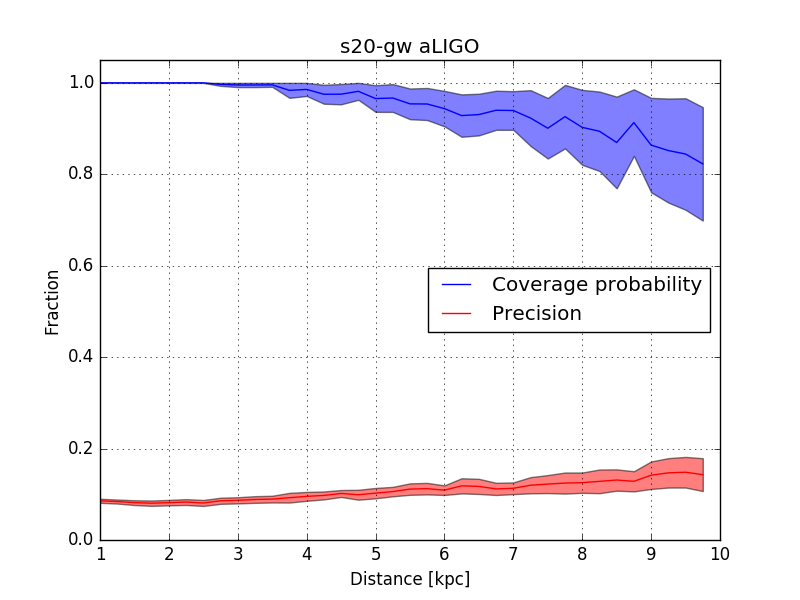
\includegraphics[width=0.5\textwidth]{plots/s20-gw_covpbb_prec_aLIGO}
 \caption{$covpbb$ and $precision$ for {\tt s20-gw-10kpc} signal embedded in aLIGO noise at different distance from the Earth. The shaded regions are given by the median absolute deviation.} \label{fig:s20results}
\end{figure}


\begin{figure}
 \centering
 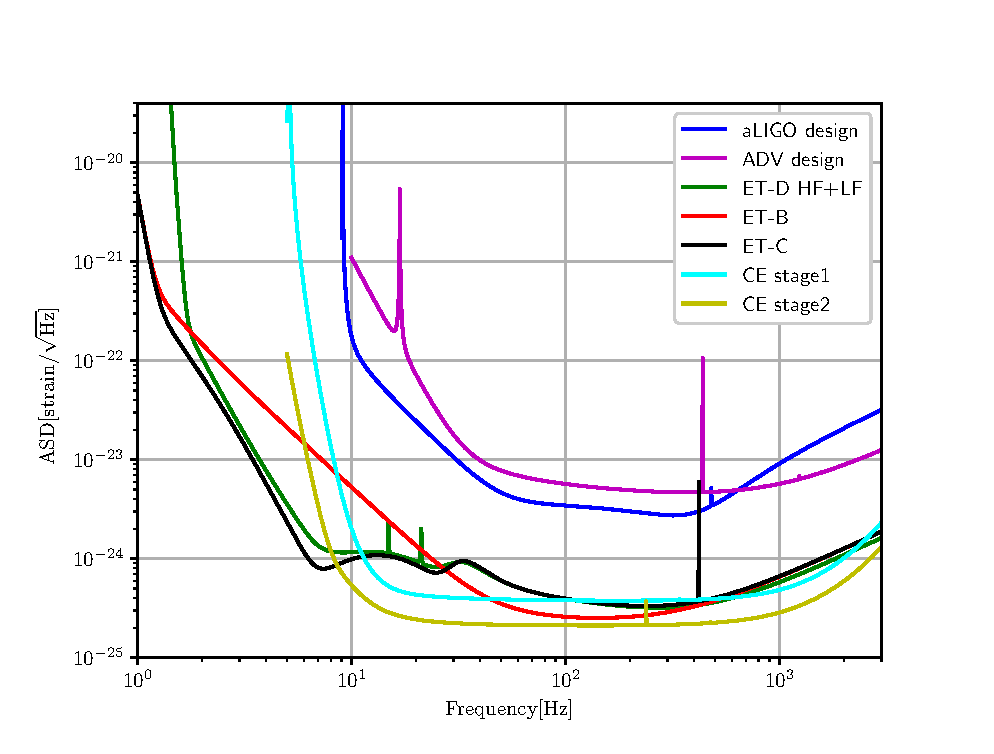
\includegraphics[width=0.5\textwidth]{plots/spectrum}
 \caption{} \label{fig:spectrum}
\end{figure}

\begin{figure}
  \centering
  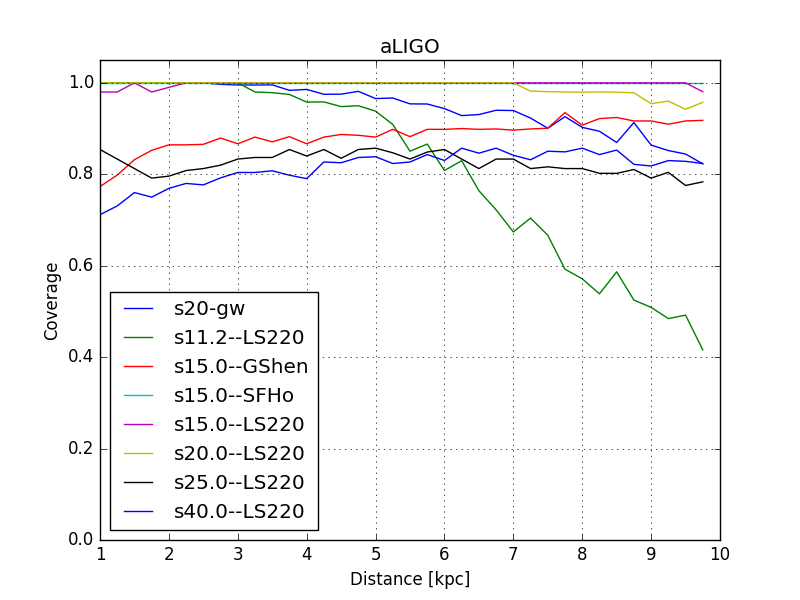
\includegraphics[width=0.5\textwidth]{plots/covppb_all_aLIGO}
 \caption{$covpbb$ for 7 waveforms embedded in aLIGO noise at different distance from the Earth. } \label{fig:aLIGOall}
\end{figure}

